\documentclass{minimal}
\usepackage{mathtools}
\usepackage{tikz}
\usetikzlibrary{tikzmark,calc,fit}

\begin{document}

\begin{equation*}
y=\tikzmark{mark1}m\tikzmark{mark2} \cdot x + \tikzmark{mark3}q\tikzmark{mark4}
\end{equation*}
\vspace{1cm}
\begin{tikzpicture}[overlay,remember picture]

 \node [fit=(pic cs:mark1)(pic cs:mark2),inner sep=2pt,minimum height=3ex,yshift=0.5ex,blue!20,draw,thick,rounded corners] (a) {};
 \node [fit=(pic cs:mark3)(pic cs:mark4),inner sep=2pt,minimum height=3ex,yshift=0.5ex,red!20,draw,thick,rounded corners] (b) {};

 \draw [->] (a) to[bend left] ++(2,1) node[right] {angular coefficient};
 \draw [->] (b) to[bend right] ++(1,-1) node[right] {$y$-intercept};
\end{tikzpicture}
\begin{equation*}
y=\tikzmark{mark1}m\tikzmark{mark2} \cdot x + \tikzmark{mark3}q\tikzmark{mark4}
\end{equation*}

\usetikzlibrary{positioning}

\vspace{2cm}

\begin{equation*}
     y = \tikz[baseline=(n1.base)]{\node[fill=yellow!50, draw, circle,  inner sep=1.5pt] (n1){$m$};
     \node[overlay, above right=of n1] (t1) {angular coefficient};
     \draw [overlay, ->] (n1.north) to [bend left=45] (t1.west);
     } 
    %  \hspace{-1cm}
     \cdot x +\tikz[baseline=(n2.base)]{\node[fill=green!50, draw, circle, anchor=south, inner sep=1.5pt] (n2){$q$};
     \node[overlay, below right=of n2] (t2) {$y$-intercept};
     \draw [overlay, ->] (n2.south) to [bend right=45] (t2.west);
     }
\end{equation*}

\vspace{2cm}

\begin{equation*}
y =
\tikz[baseline=(a.base)]{
    \node[circle, draw=blue, fill=blue!60, inner sep=1pt] (a) {$a$};
    \draw[overlay, blue, thick, ->] (a.north) to[out=90, in=180] +(30:1cm)
        node[anchor=west,text=black] {angular coefficient};
}
\cdot x +
\tikz[baseline=(q.base)]{
    \node[circle, draw=green, fill=green!60, inner sep=1pt] (q) {$q$};
    \draw[overlay, green, thick, ->] (a.south) to[out=-90, in=180] +(-30:1cm)
        node[anchor=west,text=black] {y-intercept};
}
\end{equation*}
\vspace{1cm}

Drawing a red node
\tikz[remember picture]{\node [circle, fill=red!50] (n1) {};}
and a blue one
\tikz[remember picture]{\node [circle, fill=blue!50] (n2) {};}.
Now, I'm drawing a curved arrow between them.
\tikz[remember picture, overlay]{\draw[->, bend left=45] (n1) to (n2);}

% \begin{tikzpicture}[remember picture, overlay, out=45,in=135]
%   \draw (n1) to (n2)
%         (0,0) to (2,0)
%         (0,0) to (3,0);
% \end{tikzpicture}

\end{document}